%# -*- coding:utf-8 -*-
\pagestyle{empty}
%\begin{document}
%\fontsize{14}{21}\selectfont

% \begin{center}\section*{\heiti \zihao{-2}厦门大学学位论文原创性声明}\end{center}
% \vspace*{21pt}
%  \par \zihao{4}
%  本人呈交的学位论文是本人在导师指导下,独立完成的研究成果。本人在论文写作中参考其他个人或集体已经发表的研究成果,均在文中以适当方式明确标明,并符合法律规范和《厦门大学研究生学术活动规范(试行)》。
%  \par
%  另外,该学位论文为(\hspace{12em})课题(组)的研究成果,获得(~~~~~~~~~~~~~~~~~~~~~~~~~~~)课题(组)经费或实验室的资助,在(~~~~~~~~~~~~~~~~~~~~~~~~~~~~~~~~~~)实验室完成。(请在以上括号内填写课题或课题组负责人或实验室名称,未有此项声明内容的,可以不作特别声明。)
%  \par
%  本人声明该学位论文不存在剽窃、抄袭等学术不端行为,并愿意承担因学术不端行为所带来的一切后果和法律责任。
%  \vspace{3ex}
%  \par \hfill
%  声明人(签名):~~~~~~~~~~~~
% \par \hfill
%  指导教师(签名):~~~~~~~~~~~~
%  \par \hfill
%  年~~~~~~~~月~~~~~~~~~日
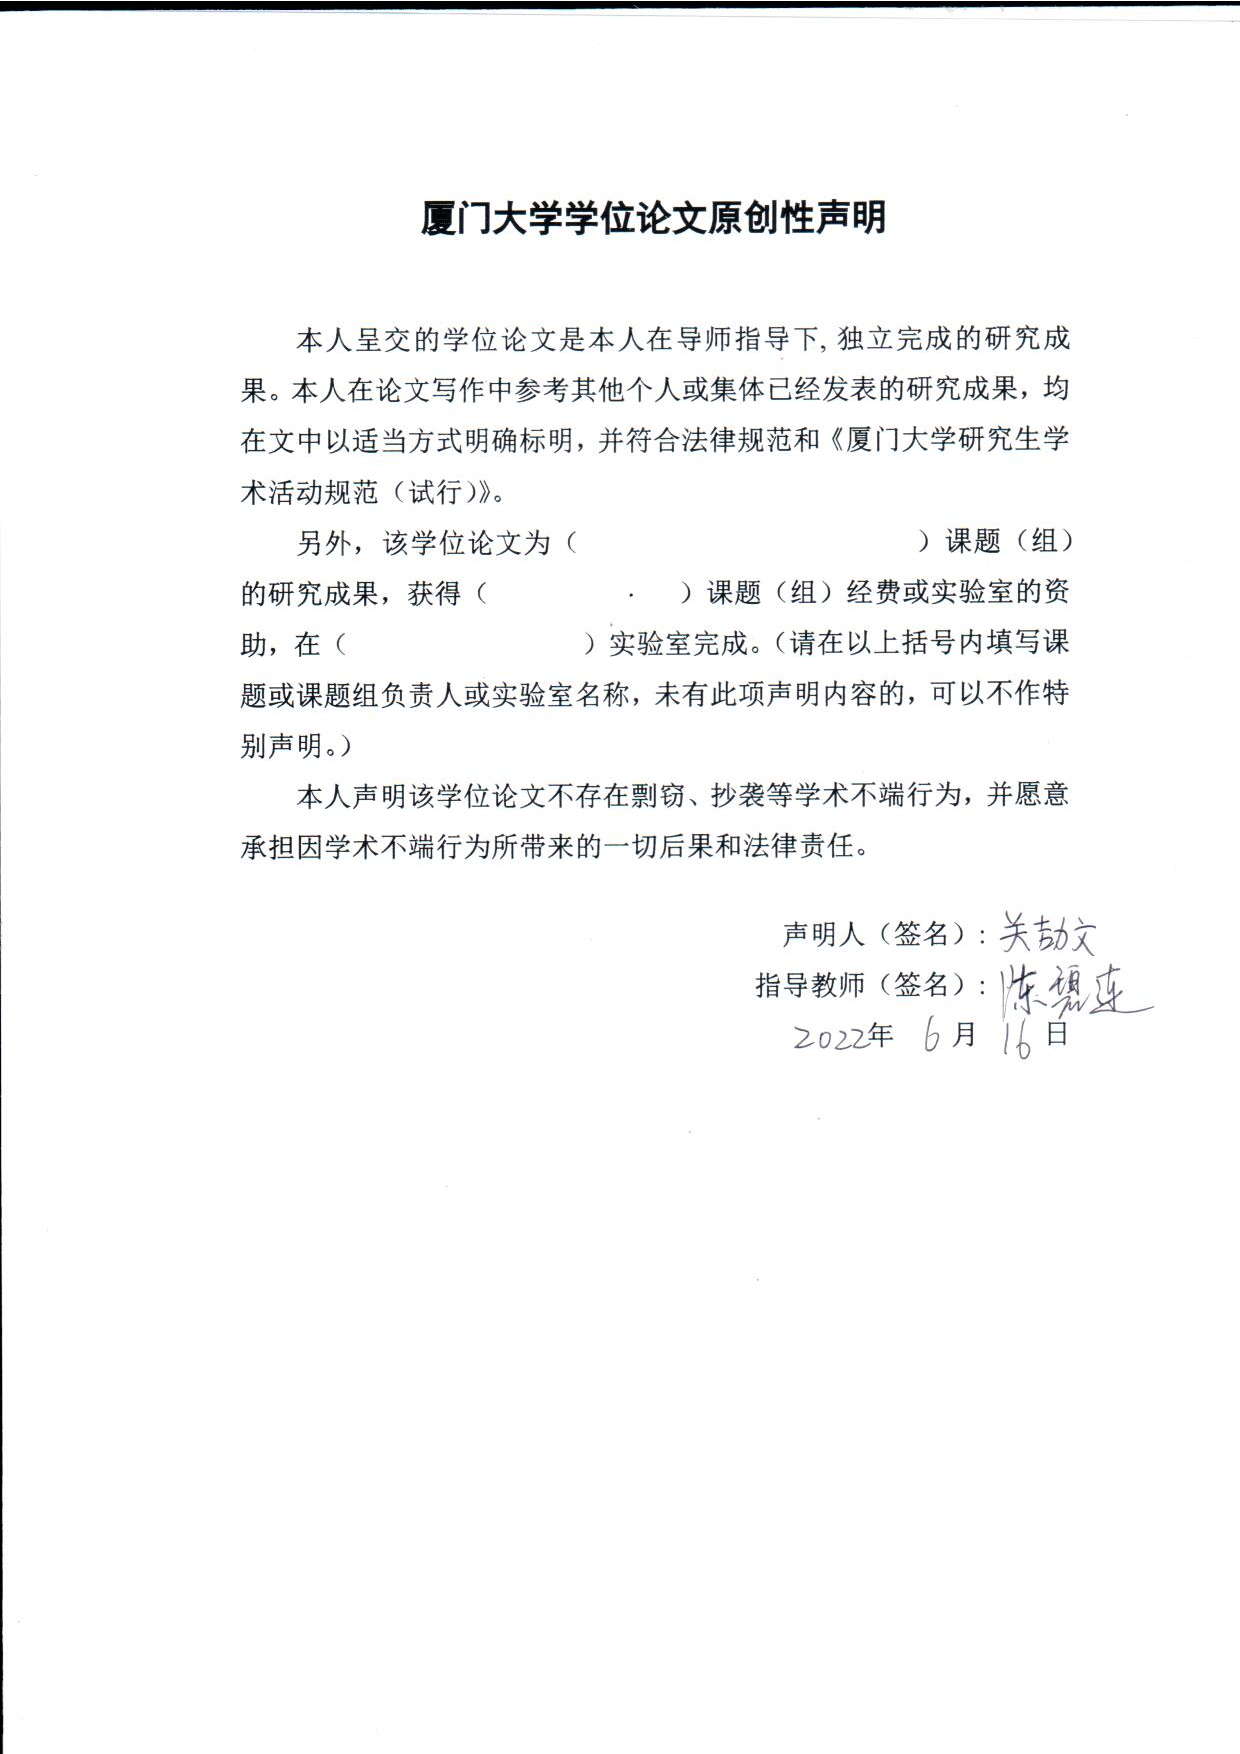
\includepdf[pages=-]{figures/yuanchuang.pdf}
%  \clearpage\cleardoublepage
\afterpage{\null\newpage}\clearpage

% \begin{center}\section*{\heiti \zihao{-2}厦门大学学位论文著作权使用声明}\end{center}
% \vspace*{21pt}
%  \par
%  本人同意厦门大学根据《中华人民共和国学位条例暂行实施办法》等规定保留和使用此学位论文,并向主管部门或其指定机构送交学位论文(包括纸质版和电子版),允许学位论文进入厦门大学图书馆及其数据库被查阅、借阅。本人同意厦门大学将学位论文加入全国博士、硕士学位论文共建单位数据库进行检索,将学位论文的标题和摘要汇编出版,采用影印、缩印或者其它方式合理复制学位论文。
%  \par
%  本学位论文属于:
%  \par
%  \thinspace(\hspace{3em})1.经厦门大学保密委员会审查核定的保密学位论文,于\quad \qquad 年\qquad 月\qquad 日解密,解密后适用上述授权。
%  \par
%  \thinspace(\hspace{3em})2.不保密,适用上述授权。
%  \par
%  (请在以上相应括号内打“\checkmark”或填上相应内容。保密学位论文应是已经厦门大学保密委员会审定过的学位论文,未经厦门大学保密委员会审定的学位论文均为公开学位论文。此声明栏不填写的,默认为公开学位论文,均适用上述授权。)
%  \vspace{3ex}
%  \par \hfill
%  声明人(签名):~~~~~~~~~~~~
%  \par \hfill
%  年~~~~~~~~月~~~~~~~~~日
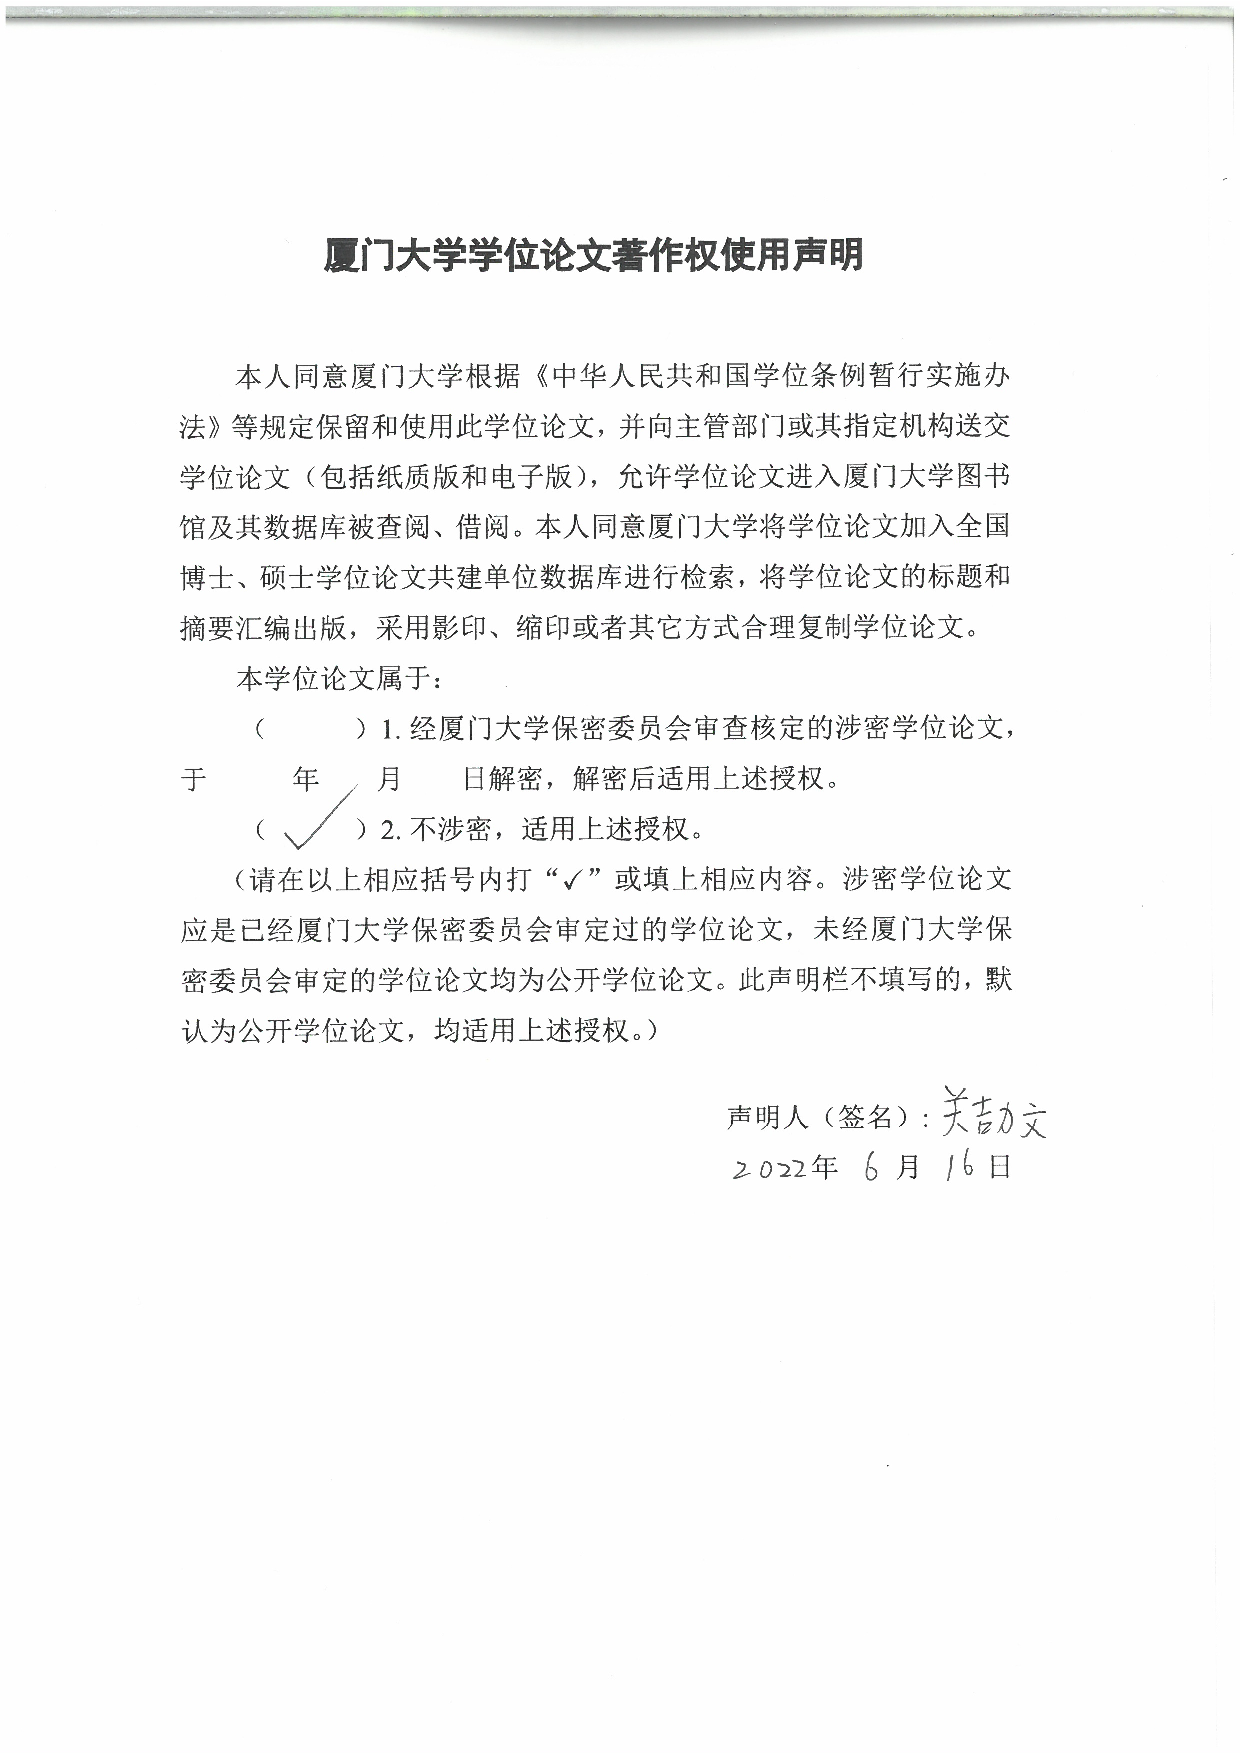
\includepdf[pages=-]{figures/zhuzuo.pdf}
\afterpage{\null\newpage}\clearpage